\documentclass[a4paper]{article}

%% Language and font encodings
\usepackage[english]{babel} 
\usepackage[utf8x]{inputenc} 
\usepackage[T1]{fontenc}

%% Sets page size and margins
\usepackage[a4paper,top=1.5cm,bottom=2cm,left=2cm,right=2cm,marginparwidth=1.75cm]{geometry}

%% Useful packages
\usepackage{amsmath,subcaption,amsfonts} 
\usepackage{graphicx} 
\usepackage[colorinlistoftodos]{todonotes} 
\usepackage[colorlinks=true, allcolors=blue]{hyperref} 
\title{Cell-centred model of an epithelium} 
\author{Jessie Renton}

\begin{document} 
\maketitle

Epithelia are the tissues which form the surfaces of our bodies and linings of organs. They consist of sheets of polygonal cells which undergo processes of proliferation, apoptosis and motility. Rates of cell replacement in epithelia tend to be much higher than in other tissues and the majority of cancers originate in epithelial cells. The dynamics of mutant invasion in epithelia is therefore of particular interest medically.

In modelling invasion on epithelia it is important to note that they are dynamic structures. While stuctural characteristics such as polygon distribution are conserved over time; cell division, apoptosis and motility lead to local stuctural changes, neighbour exchange and mixing. We suggest that a traditional evolutionary graph theory (EGT) approach is not appropriate as it is based on the use of static graphs which cannot account for this type of behaviour. Further in EGT it is necessary to couple birth and death processes in a way that is unrealistic and introduces a troubling dependence on the exact implimentation of this coupling. 

As an alternative we will use an explicit, individual-based model for epithelia. There are a number of on- and off-lattice models to choose from. We focus on the Voronoi Tesselation model for several reasons: local cell processes do not lead to global reconfigerations as in cellular automota models; it lends itself natural to a graph description of the the structure; it is described entirely by cell-centre positions.

\section{Voronoi Tesselation model}

This model is part of a class of cell-centre models in which a tissue is represented by a set of points corresponding to the centres of individual cells. These cells move freely in space and exert forces on one another. Different models in this class are characterised by the force laws and the mechanism for determining cell neighbours. Here we broadly follow the [Meinke] model with some adjustments from [Leeuwen].

\begin{figure}[htbp]
	\centering
		\frame{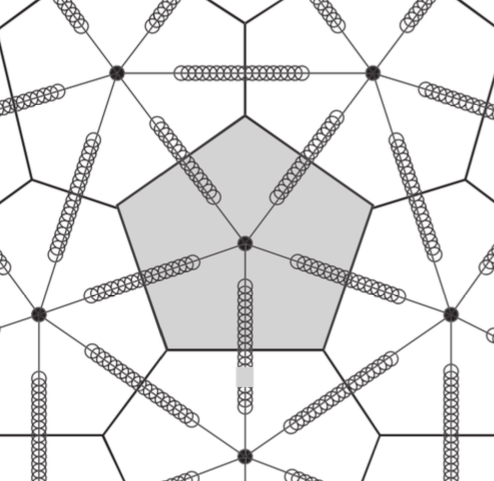
\includegraphics[width=0.4\textwidth]{springs.png}}
	\caption{Schematic of Voronoi Tesselation model: depicts cell centres and the spring-like forces exerted between their neighburs as obtained from the Delaunay Triangulation. Also shown are the cell shapes defined by the Voronoi region of each cell-centre. [Leeuwen]}
	\label{fig:spring}
\end{figure} 
\subsection{Force law}
The assumption in this model is that cells act as if they are connected to their neighbours by a network of springs, such that 
\begin{equation} \mathbf{F}_{ij}(t) = \mu_{ij}\hat{\mathbf{r}}_{ij}(t)(\vert \mathbf{r}_{ij}(t) \vert -s_{ij}(t))
	\end{equation}
is the force exerted by cell $j$ on its neighbour $i$. Here $\mu_{ij}$ are the spring constants and $\mathbf{r}_{ij}=\mathbf{r}_{i}-\mathbf{r}_ {j}$, where $\mathbf{r}_i$ is the position vector of cell $i$ and $\hat{\mathbf{r}}_{ij}$ is the corresponding unit vector. The natural seperation between cells $s_{ij}(t)=s$ except for newborn sister cells which have a natural seperation of $\epsilon < 1$ when they are born and this increases linearly to $s$ over 1h.

The total force acting on cell $i$ is then
\begin{equation}
	\mathbf{F}_i(t)= \sum_{j \in \mathcal{N}_i(t)}\mathbf{F}_{ij}
\end{equation}
where $\mathcal{N}_i(t)$ is the set of cells neighbouring $i$.

By assuming that motion is overdamped due to high levels of friction we obtain the equation of motion for each cell in the form of a first order differential equation
\begin{equation}
	\eta \frac{d\mathbf{r}_i}{dt}= \mathbf{F}_i(t)
\end{equation}
where $\eta$ is the damping constant. This is solved numerically using
\begin{equation}
	\mathbf{r}_i(t+\delta t)= \mathbf{r}_i(t)+\frac{\delta t}{\eta} \mathbf{F}_i
\end{equation}

where $\delta t$ is a sufficiently small time step for numerical stability.
\subsection{Neighbours}
In the VT model we define the neighbour connections between cells to be the Delaunay Triangulation (DT) on the set of cell-centres. The dual of the DT is the Voronoi Tesselation which divides the plane into polygons, where each polygon is defined as the the region of the plane closest to its generator (i.e. cell-centre) than any other. Each cell can therefore be represented as a distinct region with a well-defined area (except on the boundary). 

As the VT/DT are defined by the cell-centre positions, they must be recalculated after every timestep.


\subsection{Cell division and extrusion}
When a cell divides its cell-centre is removed and replaced with two new cell-centres. These are placed a small distance $\epsilon$ from each other, equidistant from their mother across a random axis. 

\begin{figure}[htbp]
\centering
\begin{subfigure}{0.24\textwidth}
	\centering
	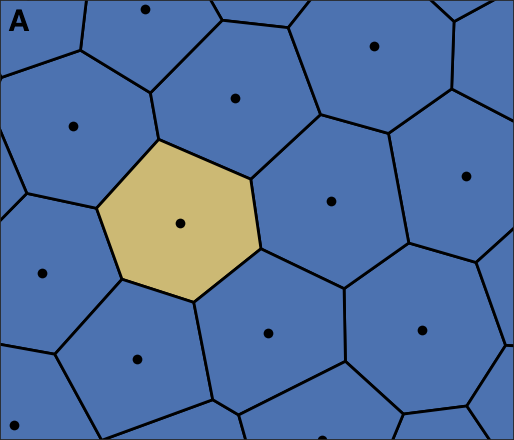
\includegraphics[width=3.7cm]{divide_1.png}
	\label{fig:divideA}
\end{subfigure} \hspace{0.02cm}
\centering
\begin{subfigure}{0.24\textwidth}
	\centering
	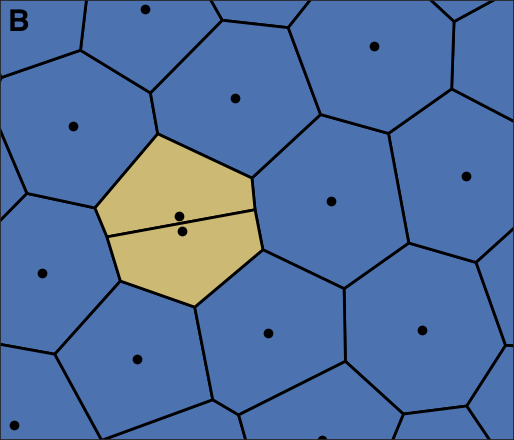
\includegraphics[width=3.7cm]{divide_2.png}
	\label{fig:divideA}
\end{subfigure} \hspace{0.02cm}
\centering
\begin{subfigure}{0.24\textwidth}
	\centering
	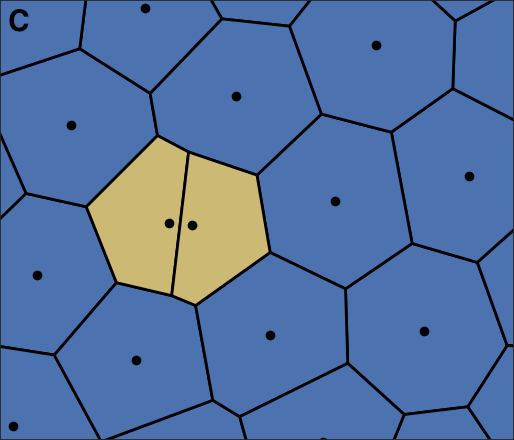
\includegraphics[width=3.7cm]{divide_3.png}
	\label{fig:divideA}
\end{subfigure} \hspace{0.02cm}
\centering
\begin{subfigure}{0.24\textwidth}
	\centering
	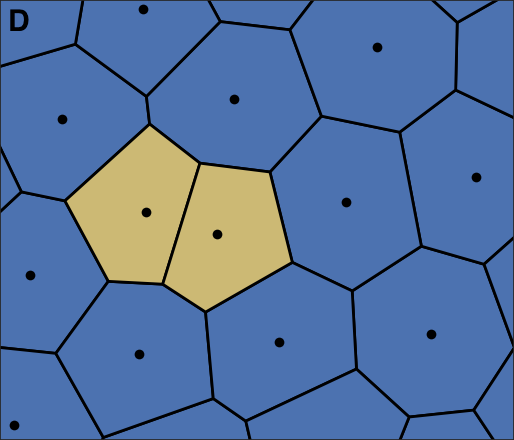
\includegraphics[width=3.7cm]{divide_4.png}
	\label{fig:divideA}
\end{subfigure} \\
\caption{Cell division}
\label{fig:manmade}
\end{figure}
When a cell is extruded from the tissue cell-centre is removed.

\begin{figure}[htbp]
\centering
\begin{subfigure}{0.24\textwidth}
	\centering
	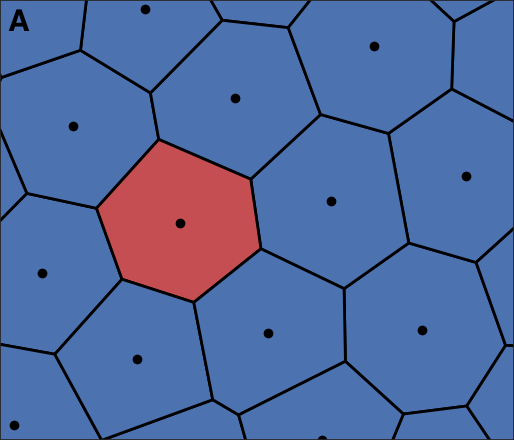
\includegraphics[width=3.7cm]{dead_1.png}
	\label{fig:divideA}
\end{subfigure} \hspace{0.02cm}
\centering
\begin{subfigure}{0.24\textwidth}
	\centering
	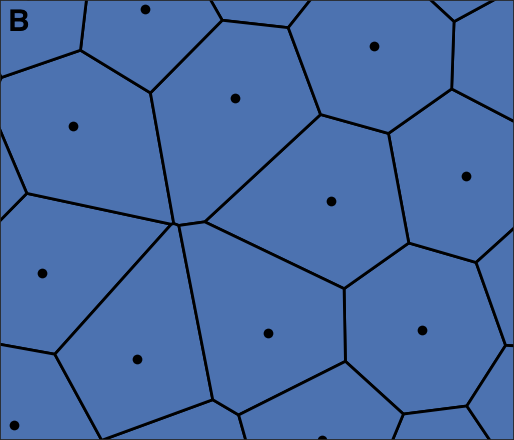
\includegraphics[width=3.7cm]{dead_2.png}
	\label{fig:divideA}
\end{subfigure} \hspace{0.02cm}
\centering
\begin{subfigure}{0.24\textwidth}
	\centering
	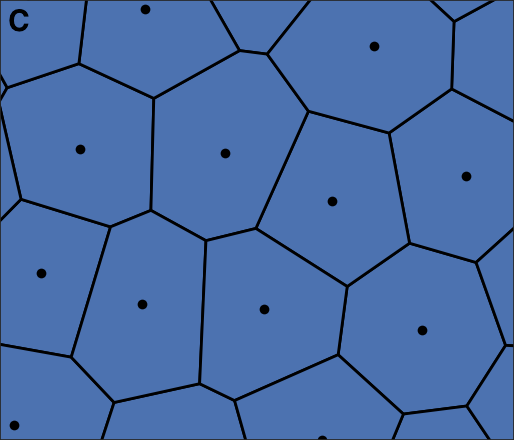
\includegraphics[width=3.7cm]{dead_3.png}
	\label{fig:divideA}
\end{subfigure}
\caption{Cell extrusion}
\label{fig:manmade}
\end{figure}

\subsection{Simulation}
The simulation algorithm proceeds as follows: (1) DT is performed to determine cell neighbours; (2) forces are calculated and the cells moved accordingly; (3) any cells at the end of their cycle divide; (4) cell death if applicable; (5) cells age.

\subsection{Boundary}
Voronoi Tesselation results in boundary cells with very large or infinite area which correspond to

\section{Implementation}
Currently there are a number of problems with implement
 
\bibliographystyle{ieeetr} 
\bibliography{sample}

\end{document}
